\documentclass[12pt]{article}
\usepackage{tikz}
\usepackage{amsmath}
% Underlining package
\usepackage{ulem}
\usetikzlibrary{calc}
\usepackage[a4paper, portrait, margin=1cm]{geometry}
\usepackage{fancyhdr}

\def \HeadingAnswers {\section*{\Large Name: \underline{\hspace{8cm}} \hfill Date: \underline{\hspace{3cm}}} \vspace{-3mm}
{Angles in a Triangle: Answers} \vspace{1pt}\hrule}

% raise footer with page number; no header
\fancypagestyle{myfancypagestyle}{
  \fancyhf{}% clear all header and footer fields
  \renewcommand{\headrulewidth}{0pt} % no rule under header
  \fancyfoot[C] {\thepage} \setlength{\footskip}{14.5pt} % raise page number allowed min 14.5pt
}
\pagestyle{myfancypagestyle}  % apply myfancypagestyle

\newcounter{minipagecount}

\begin{document}
\HeadingAnswers
\vspace{8mm}

\begin{minipage}{0.55\textwidth}
  \refstepcounter{minipagecount}
  \noindent{(\theminipagecount)}\quad
  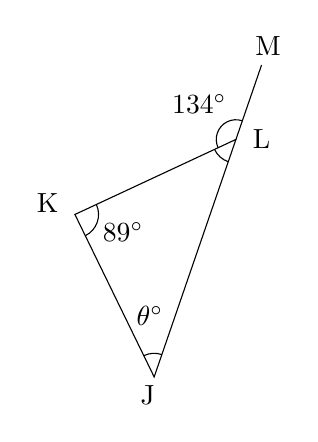
\begin{tikzpicture}[scale=1.0, baseline=(current bounding box.north)]

      \begin{scope}[rotate=71]
        \coordinate (A) at (0,0);
        \coordinate (B) at (3.189997905219,0);
        \coordinate (D) at (4.189997905219,0);
        \coordinate (C) at (intersection cs: first line={(A)--($(A)+(45:4cm)$)}, second line={(B)--($(B)+(180-46:4cm)$)});
        \draw (A) -- (B) -- (C) -- cycle;
        \draw (B) -- (D);

        % Mark angles with arcs
        \draw ($(A)!0.3cm!(B)$) arc [start angle=0, end angle=45, radius=0.3cm];
        \draw ($(B)!0.3cm!(C)$) arc [start angle=180-46, end angle=180, radius=0.3cm];
        \draw ($(C)!0.3cm!(A)$) arc [start angle=180+45, end angle=360-46, radius=0.3cm];
        \draw ($(B)!0.25cm!(D)$) arc [start angle=0, end angle=180-46, radius=0.25cm];

        % Label angles
        \node at ($(A)!-0.25cm!(B)$) {J};
        \node at ($(B)!-0.45cm!(C)!0.2cm!(A)$) {L};
        \node at ($(C)!-0.25cm!(A)!-0.25cm!(B)$) {K};
        \node at ($(D)!-0.25cm!(A)$) {M};

        % Mark angles in degrees
        \coordinate (midBC) at ($(B)!0.5!(C)$);
        \node at ($(A)!0.70cm!(midBC)!0.10cm!(C)$) {$\theta^\circ$};

        \coordinate (midAC) at ($(A)!0.5!(C)$);
        \node at ($(B)!0.65cm!(midAC)$) {};

        \coordinate (midAB) at ($(A)!0.5!(B)$);
        \node at ($(C)!0.65cm!(midAB)$) {$89^\circ$};

        \coordinate (midDC) at ($(D)!0.3!(C)$);
        \node at ($(B)!0.65cm!(midDC)$) {$134^\circ$};


      \end{scope}
    \end{tikzpicture}
\end{minipage}%
\hfill
\begin{minipage}{0.4\textwidth}
  \begin{align*}
    \angle \text{J} &= \angle \text{MLK} - \angle \text{K} \\
    &= 134^\circ  - 89^\circ \\
    &= 45^\circ
  \end{align*}
\end{minipage}
\vspace{1cm} \vfill\begin{minipage}{0.55\textwidth}
  \refstepcounter{minipagecount}
  \noindent{(\theminipagecount)}\quad
  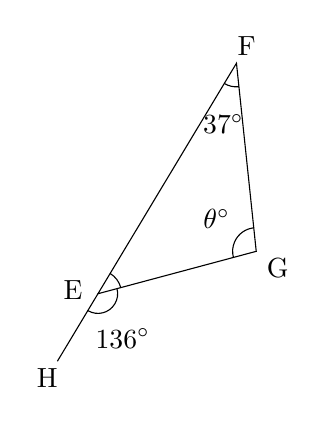
\begin{tikzpicture}[scale=1.0, baseline=(current bounding box.north)]

      \begin{scope}[rotate=239]
        \coordinate (A) at (0,0);
        \coordinate (B) at (3.415059163194597,0);
        \coordinate (D) at (4.415059163194597,0);
        \coordinate (C) at (intersection cs: first line={(A)--($(A)+(37:4cm)$)}, second line={(B)--($(B)+(180-44:4cm)$)});
        \draw (A) -- (B) -- (C) -- cycle;
        \draw (B) -- (D);

        % Mark angles with arcs
        \draw ($(A)!0.3cm!(B)$) arc [start angle=0, end angle=37, radius=0.3cm];
        \draw ($(B)!0.3cm!(C)$) arc [start angle=180-44, end angle=180, radius=0.3cm];
        \draw ($(C)!0.3cm!(A)$) arc [start angle=180+37, end angle=360-44, radius=0.3cm];
        \draw ($(B)!0.25cm!(D)$) arc [start angle=0, end angle=180-44, radius=0.25cm];

        % Label angles
        \node at ($(A)!-0.25cm!(B)$) {F};
        \node at ($(B)!-0.45cm!(C)!0.2cm!(A)$) {E};
        \node at ($(C)!-0.25cm!(A)!-0.25cm!(B)$) {G};
        \node at ($(D)!-0.25cm!(A)$) {H};

        % Mark angles in degrees
        \coordinate (midBC) at ($(B)!0.5!(C)$);
        \node at ($(A)!0.70cm!(midBC)!0.10cm!(C)$) {$37^\circ$};

        \coordinate (midAC) at ($(A)!0.5!(C)$);
        \node at ($(B)!0.65cm!(midAC)$) {};

        \coordinate (midAB) at ($(A)!0.5!(B)$);
        \node at ($(C)!0.65cm!(midAB)$) {$\theta^\circ$};

        \coordinate (midDC) at ($(D)!0.3!(C)$);
        \node at ($(B)!0.65cm!(midDC)$) {$136^\circ$};


      \end{scope}
    \end{tikzpicture}
\end{minipage}%
\hfill
\begin{minipage}{0.4\textwidth}
  \begin{align*}
    \angle \text{G} &= \angle \text{HEG} - \angle \text{F} \\
    &= 136^\circ  - 37^\circ \\
    &= 99^\circ
  \end{align*}
\end{minipage}
\vspace{1cm} \vfill\begin{minipage}{0.55\textwidth}
  \refstepcounter{minipagecount}
  \noindent{(\theminipagecount)}\quad
  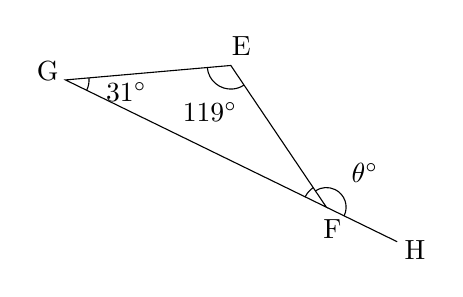
\begin{tikzpicture}[scale=1.0, baseline=(current bounding box.north)]

      \begin{scope}[rotate=334]
        \coordinate (A) at (0,0);
        \coordinate (B) at (3.6876280291617802,0);
        \coordinate (D) at (4.687628029161781,0);
        \coordinate (C) at (intersection cs: first line={(A)--($(A)+(31:4cm)$)}, second line={(B)--($(B)+(180-30:4cm)$)});
        \draw (A) -- (B) -- (C) -- cycle;
        \draw (B) -- (D);

        % Mark angles with arcs
        \draw ($(A)!0.3cm!(B)$) arc [start angle=0, end angle=31, radius=0.3cm];
        \draw ($(B)!0.3cm!(C)$) arc [start angle=180-30, end angle=180, radius=0.3cm];
        \draw ($(C)!0.3cm!(A)$) arc [start angle=180+31, end angle=360-30, radius=0.3cm];
        \draw ($(B)!0.25cm!(D)$) arc [start angle=0, end angle=180-30, radius=0.25cm];

        % Label angles
        \node at ($(A)!-0.25cm!(B)$) {G};
        \node at ($(B)!-0.45cm!(C)!0.2cm!(A)$) {F};
        \node at ($(C)!-0.25cm!(A)!-0.25cm!(B)$) {E};
        \node at ($(D)!-0.25cm!(A)$) {H};

        % Mark angles in degrees
        \coordinate (midBC) at ($(B)!0.5!(C)$);
        \node at ($(A)!0.70cm!(midBC)!0.10cm!(C)$) {$31^\circ$};

        \coordinate (midAC) at ($(A)!0.5!(C)$);
        \node at ($(B)!0.65cm!(midAC)$) {};

        \coordinate (midAB) at ($(A)!0.5!(B)$);
        \node at ($(C)!0.65cm!(midAB)$) {$119^\circ$};

        \coordinate (midDC) at ($(D)!0.3!(C)$);
        \node at ($(B)!0.65cm!(midDC)$) {$\theta^\circ$};


      \end{scope}
    \end{tikzpicture}
\end{minipage}%
\hfill
\begin{minipage}{0.4\textwidth}
  \begin{align*}
    \angle \text{HFE} &= \angle \text{G} + \angle \text{E} \\
    &= 31^\circ  + 119^\circ \\
    &= 150^\circ
  \end{align*}
\end{minipage}
\vspace{1cm} \vfill\begin{minipage}{0.55\textwidth}
  \refstepcounter{minipagecount}
  \noindent{(\theminipagecount)}\quad
  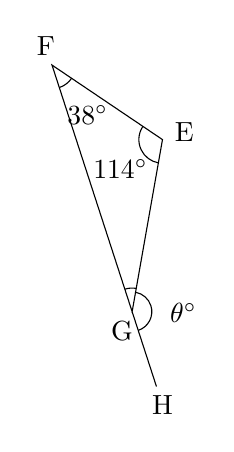
\begin{tikzpicture}[scale=1.0, baseline=(current bounding box.north)]

      \begin{scope}[rotate=288]
        \coordinate (A) at (0,0);
        \coordinate (B) at (3.292773961057914,0);
        \coordinate (D) at (4.2927739610579145,0);
        \coordinate (C) at (intersection cs: first line={(A)--($(A)+(38:4cm)$)}, second line={(B)--($(B)+(180-28:4cm)$)});
        \draw (A) -- (B) -- (C) -- cycle;
        \draw (B) -- (D);

        % Mark angles with arcs
        \draw ($(A)!0.3cm!(B)$) arc [start angle=0, end angle=38, radius=0.3cm];
        \draw ($(B)!0.3cm!(C)$) arc [start angle=180-28, end angle=180, radius=0.3cm];
        \draw ($(C)!0.3cm!(A)$) arc [start angle=180+38, end angle=360-28, radius=0.3cm];
        \draw ($(B)!0.25cm!(D)$) arc [start angle=0, end angle=180-28, radius=0.25cm];

        % Label angles
        \node at ($(A)!-0.25cm!(B)$) {F};
        \node at ($(B)!-0.45cm!(C)!0.2cm!(A)$) {G};
        \node at ($(C)!-0.25cm!(A)!-0.25cm!(B)$) {E};
        \node at ($(D)!-0.25cm!(A)$) {H};

        % Mark angles in degrees
        \coordinate (midBC) at ($(B)!0.5!(C)$);
        \node at ($(A)!0.70cm!(midBC)!0.10cm!(C)$) {$38^\circ$};

        \coordinate (midAC) at ($(A)!0.5!(C)$);
        \node at ($(B)!0.65cm!(midAC)$) {};

        \coordinate (midAB) at ($(A)!0.5!(B)$);
        \node at ($(C)!0.65cm!(midAB)$) {$114^\circ$};

        \coordinate (midDC) at ($(D)!0.3!(C)$);
        \node at ($(B)!0.65cm!(midDC)$) {$\theta^\circ$};


      \end{scope}
    \end{tikzpicture}
\end{minipage}%
\hfill
\begin{minipage}{0.4\textwidth}
  \begin{align*}
    \angle \text{HGE} &= \angle \text{F} + \angle \text{E} \\
    &= 38^\circ  + 114^\circ \\
    &= 152^\circ
  \end{align*}
\end{minipage}
\vspace{1cm} \vfill\pagebreak ~ \newline ~ \newline\begin{minipage}{0.55\textwidth}
  \refstepcounter{minipagecount}
  \noindent{(\theminipagecount)}\quad
  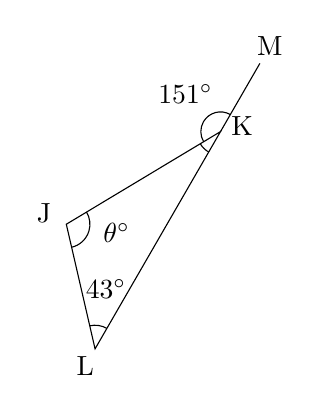
\begin{tikzpicture}[scale=1.0, baseline=(current bounding box.north)]

      \begin{scope}[rotate=60]
        \coordinate (A) at (0,0);
        \coordinate (B) at (3.1860813171431133,0);
        \coordinate (D) at (4.186081317143113,0);
        \coordinate (C) at (intersection cs: first line={(A)--($(A)+(43:4cm)$)}, second line={(B)--($(B)+(180-29:4cm)$)});
        \draw (A) -- (B) -- (C) -- cycle;
        \draw (B) -- (D);

        % Mark angles with arcs
        \draw ($(A)!0.3cm!(B)$) arc [start angle=0, end angle=43, radius=0.3cm];
        \draw ($(B)!0.3cm!(C)$) arc [start angle=180-29, end angle=180, radius=0.3cm];
        \draw ($(C)!0.3cm!(A)$) arc [start angle=180+43, end angle=360-29, radius=0.3cm];
        \draw ($(B)!0.25cm!(D)$) arc [start angle=0, end angle=180-29, radius=0.25cm];

        % Label angles
        \node at ($(A)!-0.25cm!(B)$) {L};
        \node at ($(B)!-0.45cm!(C)!0.2cm!(A)$) {K};
        \node at ($(C)!-0.25cm!(A)!-0.25cm!(B)$) {J};
        \node at ($(D)!-0.25cm!(A)$) {M};

        % Mark angles in degrees
        \coordinate (midBC) at ($(B)!0.5!(C)$);
        \node at ($(A)!0.70cm!(midBC)!0.10cm!(C)$) {$43^\circ$};

        \coordinate (midAC) at ($(A)!0.5!(C)$);
        \node at ($(B)!0.65cm!(midAC)$) {};

        \coordinate (midAB) at ($(A)!0.5!(B)$);
        \node at ($(C)!0.65cm!(midAB)$) {$\theta^\circ$};

        \coordinate (midDC) at ($(D)!0.3!(C)$);
        \node at ($(B)!0.65cm!(midDC)$) {$151^\circ$};


      \end{scope}
    \end{tikzpicture}
\end{minipage}%
\hfill
\begin{minipage}{0.4\textwidth}
  \begin{align*}
    \angle \text{J} &= \angle \text{MKJ} - \angle \text{L} \\
    &= 151^\circ  - 43^\circ \\
    &= 108^\circ
  \end{align*}
\end{minipage}
\vspace{1cm} \vfill\begin{minipage}{0.55\textwidth}
  \refstepcounter{minipagecount}
  \noindent{(\theminipagecount)}\quad
  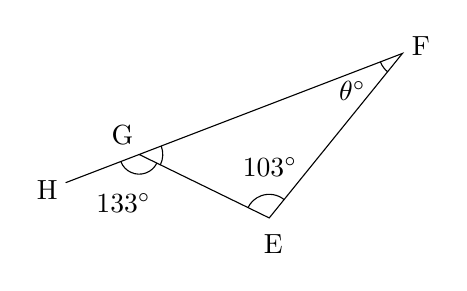
\begin{tikzpicture}[scale=1.0, baseline=(current bounding box.north)]

      \begin{scope}[rotate=201]
        \coordinate (A) at (0,0);
        \coordinate (B) at (3.5817689638456294,0);
        \coordinate (D) at (4.581768963845629,0);
        \coordinate (C) at (intersection cs: first line={(A)--($(A)+(30:4cm)$)}, second line={(B)--($(B)+(180-47:4cm)$)});
        \draw (A) -- (B) -- (C) -- cycle;
        \draw (B) -- (D);

        % Mark angles with arcs
        \draw ($(A)!0.3cm!(B)$) arc [start angle=0, end angle=30, radius=0.3cm];
        \draw ($(B)!0.3cm!(C)$) arc [start angle=180-47, end angle=180, radius=0.3cm];
        \draw ($(C)!0.3cm!(A)$) arc [start angle=180+30, end angle=360-47, radius=0.3cm];
        \draw ($(B)!0.25cm!(D)$) arc [start angle=0, end angle=180-47, radius=0.25cm];

        % Label angles
        \node at ($(A)!-0.25cm!(B)$) {F};
        \node at ($(B)!-0.45cm!(C)!0.2cm!(A)$) {G};
        \node at ($(C)!-0.25cm!(A)!-0.25cm!(B)$) {E};
        \node at ($(D)!-0.25cm!(A)$) {H};

        % Mark angles in degrees
        \coordinate (midBC) at ($(B)!0.5!(C)$);
        \node at ($(A)!0.70cm!(midBC)!0.10cm!(C)$) {$\theta^\circ$};

        \coordinate (midAC) at ($(A)!0.5!(C)$);
        \node at ($(B)!0.65cm!(midAC)$) {};

        \coordinate (midAB) at ($(A)!0.5!(B)$);
        \node at ($(C)!0.65cm!(midAB)$) {$103^\circ$};

        \coordinate (midDC) at ($(D)!0.3!(C)$);
        \node at ($(B)!0.65cm!(midDC)$) {$133^\circ$};


      \end{scope}
    \end{tikzpicture}
\end{minipage}%
\hfill
\begin{minipage}{0.4\textwidth}
  \begin{align*}
    \angle \text{F} &= \angle \text{HGE} - \angle \text{E} \\
    &= 133^\circ  - 103^\circ \\
    &= 30^\circ
  \end{align*}
\end{minipage}
\vspace{1cm} \vfill\begin{minipage}{0.55\textwidth}
  \refstepcounter{minipagecount}
  \noindent{(\theminipagecount)}\quad
  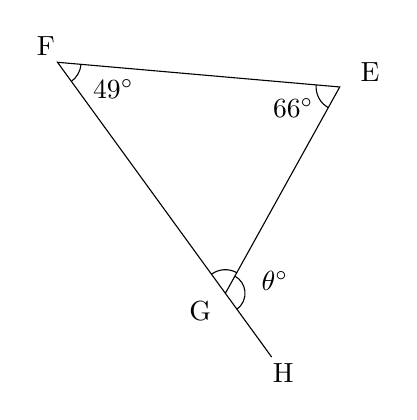
\begin{tikzpicture}[scale=1.0, baseline=(current bounding box.north)]

      \begin{scope}[rotate=306]
        \coordinate (A) at (0,0);
        \coordinate (B) at (3.626749494584979,0);
        \coordinate (D) at (4.626749494584979,0);
        \coordinate (C) at (intersection cs: first line={(A)--($(A)+(49:4cm)$)}, second line={(B)--($(B)+(180-65:4cm)$)});
        \draw (A) -- (B) -- (C) -- cycle;
        \draw (B) -- (D);

        % Mark angles with arcs
        \draw ($(A)!0.3cm!(B)$) arc [start angle=0, end angle=49, radius=0.3cm];
        \draw ($(B)!0.3cm!(C)$) arc [start angle=180-65, end angle=180, radius=0.3cm];
        \draw ($(C)!0.3cm!(A)$) arc [start angle=180+49, end angle=360-65, radius=0.3cm];
        \draw ($(B)!0.25cm!(D)$) arc [start angle=0, end angle=180-65, radius=0.25cm];

        % Label angles
        \node at ($(A)!-0.25cm!(B)$) {F};
        \node at ($(B)!-0.45cm!(C)!0.2cm!(A)$) {G};
        \node at ($(C)!-0.25cm!(A)!-0.25cm!(B)$) {E};
        \node at ($(D)!-0.25cm!(A)$) {H};

        % Mark angles in degrees
        \coordinate (midBC) at ($(B)!0.5!(C)$);
        \node at ($(A)!0.70cm!(midBC)!0.10cm!(C)$) {$49^\circ$};

        \coordinate (midAC) at ($(A)!0.5!(C)$);
        \node at ($(B)!0.65cm!(midAC)$) {};

        \coordinate (midAB) at ($(A)!0.5!(B)$);
        \node at ($(C)!0.65cm!(midAB)$) {$66^\circ$};

        \coordinate (midDC) at ($(D)!0.3!(C)$);
        \node at ($(B)!0.65cm!(midDC)$) {$\theta^\circ$};


      \end{scope}
    \end{tikzpicture}
\end{minipage}%
\hfill
\begin{minipage}{0.4\textwidth}
  \begin{align*}
    \angle \text{HGE} &= \angle \text{F} + \angle \text{E} \\
    &= 49^\circ  + 66^\circ \\
    &= 115^\circ
  \end{align*}
\end{minipage}
\vspace{1cm} \vfill\begin{minipage}{0.55\textwidth}
  \refstepcounter{minipagecount}
  \noindent{(\theminipagecount)}\quad
  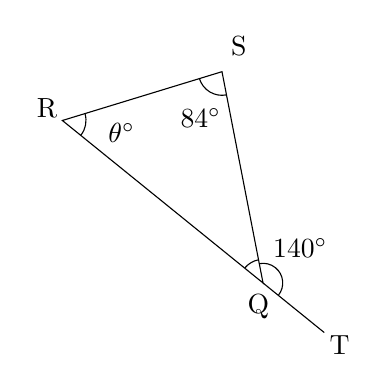
\begin{tikzpicture}[scale=1.0, baseline=(current bounding box.north)]

      \begin{scope}[rotate=321]
        \coordinate (A) at (0,0);
        \coordinate (B) at (3.279167519237965,0);
        \coordinate (D) at (4.279167519237965,0);
        \coordinate (C) at (intersection cs: first line={(A)--($(A)+(56:4cm)$)}, second line={(B)--($(B)+(180-40:4cm)$)});
        \draw (A) -- (B) -- (C) -- cycle;
        \draw (B) -- (D);

        % Mark angles with arcs
        \draw ($(A)!0.3cm!(B)$) arc [start angle=0, end angle=56, radius=0.3cm];
        \draw ($(B)!0.3cm!(C)$) arc [start angle=180-40, end angle=180, radius=0.3cm];
        \draw ($(C)!0.3cm!(A)$) arc [start angle=180+56, end angle=360-40, radius=0.3cm];
        \draw ($(B)!0.25cm!(D)$) arc [start angle=0, end angle=180-40, radius=0.25cm];

        % Label angles
        \node at ($(A)!-0.25cm!(B)$) {R};
        \node at ($(B)!-0.45cm!(C)!0.2cm!(A)$) {Q};
        \node at ($(C)!-0.25cm!(A)!-0.25cm!(B)$) {S};
        \node at ($(D)!-0.25cm!(A)$) {T};

        % Mark angles in degrees
        \coordinate (midBC) at ($(B)!0.5!(C)$);
        \node at ($(A)!0.70cm!(midBC)!0.10cm!(C)$) {$\theta^\circ$};

        \coordinate (midAC) at ($(A)!0.5!(C)$);
        \node at ($(B)!0.65cm!(midAC)$) {};

        \coordinate (midAB) at ($(A)!0.5!(B)$);
        \node at ($(C)!0.65cm!(midAB)$) {$84^\circ$};

        \coordinate (midDC) at ($(D)!0.3!(C)$);
        \node at ($(B)!0.65cm!(midDC)$) {$140^\circ$};


      \end{scope}
    \end{tikzpicture}
\end{minipage}%
\hfill
\begin{minipage}{0.4\textwidth}
  \begin{align*}
    \angle \text{R} &= \angle \text{TQS} - \angle \text{S} \\
    &= 140^\circ  - 84^\circ \\
    &= 56^\circ
  \end{align*}
\end{minipage}
\vspace{1cm} \vfill\pagebreak ~ \newline ~ \newline\begin{minipage}{0.55\textwidth}
  \refstepcounter{minipagecount}
  \noindent{(\theminipagecount)}\quad
  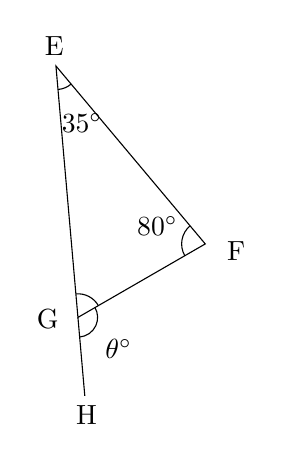
\begin{tikzpicture}[scale=1.0, baseline=(current bounding box.north)]

      \begin{scope}[rotate=275]
        \coordinate (A) at (0,0);
        \coordinate (B) at (3.2056337864672098,0);
        \coordinate (D) at (4.20563378646721,0);
        \coordinate (C) at (intersection cs: first line={(A)--($(A)+(35:4cm)$)}, second line={(B)--($(B)+(180-65:4cm)$)});
        \draw (A) -- (B) -- (C) -- cycle;
        \draw (B) -- (D);

        % Mark angles with arcs
        \draw ($(A)!0.3cm!(B)$) arc [start angle=0, end angle=35, radius=0.3cm];
        \draw ($(B)!0.3cm!(C)$) arc [start angle=180-65, end angle=180, radius=0.3cm];
        \draw ($(C)!0.3cm!(A)$) arc [start angle=180+35, end angle=360-65, radius=0.3cm];
        \draw ($(B)!0.25cm!(D)$) arc [start angle=0, end angle=180-65, radius=0.25cm];

        % Label angles
        \node at ($(A)!-0.25cm!(B)$) {E};
        \node at ($(B)!-0.45cm!(C)!0.2cm!(A)$) {G};
        \node at ($(C)!-0.25cm!(A)!-0.25cm!(B)$) {F};
        \node at ($(D)!-0.25cm!(A)$) {H};

        % Mark angles in degrees
        \coordinate (midBC) at ($(B)!0.5!(C)$);
        \node at ($(A)!0.70cm!(midBC)!0.10cm!(C)$) {$35^\circ$};

        \coordinate (midAC) at ($(A)!0.5!(C)$);
        \node at ($(B)!0.65cm!(midAC)$) {};

        \coordinate (midAB) at ($(A)!0.5!(B)$);
        \node at ($(C)!0.65cm!(midAB)$) {$80^\circ$};

        \coordinate (midDC) at ($(D)!0.3!(C)$);
        \node at ($(B)!0.65cm!(midDC)$) {$\theta^\circ$};


      \end{scope}
    \end{tikzpicture}
\end{minipage}%
\hfill
\begin{minipage}{0.4\textwidth}
  \begin{align*}
    \angle \text{HGF} &= \angle \text{E} + \angle \text{F} \\
    &= 35^\circ  + 80^\circ \\
    &= 115^\circ
  \end{align*}
\end{minipage}
\vspace{1cm} \vfill\begin{minipage}{0.55\textwidth}
  \refstepcounter{minipagecount}
  \noindent{(\theminipagecount)}\quad
  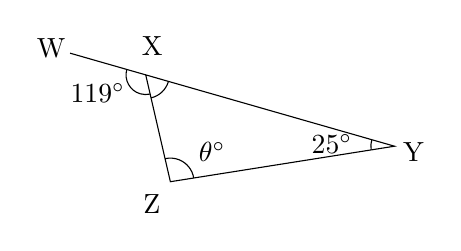
\begin{tikzpicture}[scale=1.0, baseline=(current bounding box.north)]

      \begin{scope}[rotate=164]
        \coordinate (A) at (0,0);
        \coordinate (B) at (3.2867557632058517,0);
        \coordinate (D) at (4.286755763205852,0);
        \coordinate (C) at (intersection cs: first line={(A)--($(A)+(25:4cm)$)}, second line={(B)--($(B)+(180-61:4cm)$)});
        \draw (A) -- (B) -- (C) -- cycle;
        \draw (B) -- (D);

        % Mark angles with arcs
        \draw ($(A)!0.3cm!(B)$) arc [start angle=0, end angle=25, radius=0.3cm];
        \draw ($(B)!0.3cm!(C)$) arc [start angle=180-61, end angle=180, radius=0.3cm];
        \draw ($(C)!0.3cm!(A)$) arc [start angle=180+25, end angle=360-61, radius=0.3cm];
        \draw ($(B)!0.25cm!(D)$) arc [start angle=0, end angle=180-61, radius=0.25cm];

        % Label angles
        \node at ($(A)!-0.25cm!(B)$) {Y};
        \node at ($(B)!-0.45cm!(C)!0.2cm!(A)$) {X};
        \node at ($(C)!-0.25cm!(A)!-0.25cm!(B)$) {Z};
        \node at ($(D)!-0.25cm!(A)$) {W};

        % Mark angles in degrees
        \coordinate (midBC) at ($(B)!0.5!(C)$);
        \node at ($(A)!0.70cm!(midBC)!0.10cm!(C)$) {$25^\circ$};

        \coordinate (midAC) at ($(A)!0.5!(C)$);
        \node at ($(B)!0.65cm!(midAC)$) {};

        \coordinate (midAB) at ($(A)!0.5!(B)$);
        \node at ($(C)!0.65cm!(midAB)$) {$\theta^\circ$};

        \coordinate (midDC) at ($(D)!0.3!(C)$);
        \node at ($(B)!0.65cm!(midDC)$) {$119^\circ$};


      \end{scope}
    \end{tikzpicture}
\end{minipage}%
\hfill
\begin{minipage}{0.4\textwidth}
  \begin{align*}
    \angle \text{Z} &= \angle \text{WXZ} - \angle \text{Y} \\
    &= 119^\circ  - 25^\circ \\
    &= 94^\circ
  \end{align*}
\end{minipage}
\vspace{1cm} \vfill\begin{minipage}{0.55\textwidth}
  \refstepcounter{minipagecount}
  \noindent{(\theminipagecount)}\quad
  \begin{tikzpicture}[scale=1.0, baseline=(current bounding box.north)]

      \begin{scope}[rotate=81]
        \coordinate (A) at (0,0);
        \coordinate (B) at (3.3605047994624293,0);
        \coordinate (D) at (4.360504799462429,0);
        \coordinate (C) at (intersection cs: first line={(A)--($(A)+(64:4cm)$)}, second line={(B)--($(B)+(180-56:4cm)$)});
        \draw (A) -- (B) -- (C) -- cycle;
        \draw (B) -- (D);

        % Mark angles with arcs
        \draw ($(A)!0.3cm!(B)$) arc [start angle=0, end angle=64, radius=0.3cm];
        \draw ($(B)!0.3cm!(C)$) arc [start angle=180-56, end angle=180, radius=0.3cm];
        \draw ($(C)!0.3cm!(A)$) arc [start angle=180+64, end angle=360-56, radius=0.3cm];
        \draw ($(B)!0.25cm!(D)$) arc [start angle=0, end angle=180-56, radius=0.25cm];

        % Label angles
        \node at ($(A)!-0.25cm!(B)$) {G};
        \node at ($(B)!-0.45cm!(C)!0.2cm!(A)$) {F};
        \node at ($(C)!-0.25cm!(A)!-0.25cm!(B)$) {E};
        \node at ($(D)!-0.25cm!(A)$) {H};

        % Mark angles in degrees
        \coordinate (midBC) at ($(B)!0.5!(C)$);
        \node at ($(A)!0.70cm!(midBC)!0.10cm!(C)$) {$64^\circ$};

        \coordinate (midAC) at ($(A)!0.5!(C)$);
        \node at ($(B)!0.65cm!(midAC)$) {};

        \coordinate (midAB) at ($(A)!0.5!(B)$);
        \node at ($(C)!0.65cm!(midAB)$) {$\theta^\circ$};

        \coordinate (midDC) at ($(D)!0.3!(C)$);
        \node at ($(B)!0.65cm!(midDC)$) {$124^\circ$};


      \end{scope}
    \end{tikzpicture}
\end{minipage}%
\hfill
\begin{minipage}{0.4\textwidth}
  \begin{align*}
    \angle \text{E} &= \angle \text{HFE} - \angle \text{G} \\
    &= 124^\circ  - 64^\circ \\
    &= 60^\circ
  \end{align*}
\end{minipage}
\vspace{1cm} \vfill\begin{minipage}{0.55\textwidth}
  \refstepcounter{minipagecount}
  \noindent{(\theminipagecount)}\quad
  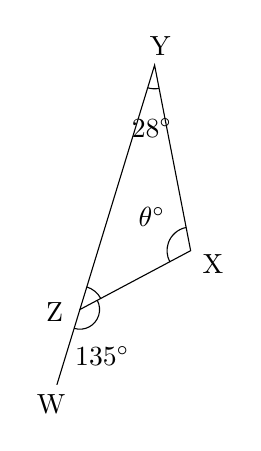
\begin{tikzpicture}[scale=1.0, baseline=(current bounding box.north)]

      \begin{scope}[rotate=253]
        \coordinate (A) at (0,0);
        \coordinate (B) at (3.2451566895853086,0);
        \coordinate (D) at (4.245156689585309,0);
        \coordinate (C) at (intersection cs: first line={(A)--($(A)+(28:4cm)$)}, second line={(B)--($(B)+(180-45:4cm)$)});
        \draw (A) -- (B) -- (C) -- cycle;
        \draw (B) -- (D);

        % Mark angles with arcs
        \draw ($(A)!0.3cm!(B)$) arc [start angle=0, end angle=28, radius=0.3cm];
        \draw ($(B)!0.3cm!(C)$) arc [start angle=180-45, end angle=180, radius=0.3cm];
        \draw ($(C)!0.3cm!(A)$) arc [start angle=180+28, end angle=360-45, radius=0.3cm];
        \draw ($(B)!0.25cm!(D)$) arc [start angle=0, end angle=180-45, radius=0.25cm];

        % Label angles
        \node at ($(A)!-0.25cm!(B)$) {Y};
        \node at ($(B)!-0.45cm!(C)!0.2cm!(A)$) {Z};
        \node at ($(C)!-0.25cm!(A)!-0.25cm!(B)$) {X};
        \node at ($(D)!-0.25cm!(A)$) {W};

        % Mark angles in degrees
        \coordinate (midBC) at ($(B)!0.5!(C)$);
        \node at ($(A)!0.70cm!(midBC)!0.10cm!(C)$) {$28^\circ$};

        \coordinate (midAC) at ($(A)!0.5!(C)$);
        \node at ($(B)!0.65cm!(midAC)$) {};

        \coordinate (midAB) at ($(A)!0.5!(B)$);
        \node at ($(C)!0.65cm!(midAB)$) {$\theta^\circ$};

        \coordinate (midDC) at ($(D)!0.3!(C)$);
        \node at ($(B)!0.65cm!(midDC)$) {$135^\circ$};


      \end{scope}
    \end{tikzpicture}
\end{minipage}%
\hfill
\begin{minipage}{0.4\textwidth}
  \begin{align*}
    \angle \text{X} &= \angle \text{WZX} - \angle \text{Y} \\
    &= 135^\circ  - 28^\circ \\
    &= 107^\circ
  \end{align*}
\end{minipage}
\vspace{1cm} \vfill\pagebreak ~ \newline ~ \newline\begin{minipage}{0.55\textwidth}
  \refstepcounter{minipagecount}
  \noindent{(\theminipagecount)}\quad
  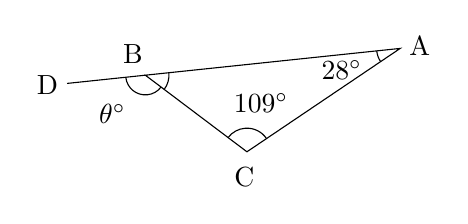
\begin{tikzpicture}[scale=1.0, baseline=(current bounding box.north)]

      \begin{scope}[rotate=186]
        \coordinate (A) at (0,0);
        \coordinate (B) at (3.254593875379487,0);
        \coordinate (D) at (4.254593875379487,0);
        \coordinate (C) at (intersection cs: first line={(A)--($(A)+(28:4cm)$)}, second line={(B)--($(B)+(180-43:4cm)$)});
        \draw (A) -- (B) -- (C) -- cycle;
        \draw (B) -- (D);

        % Mark angles with arcs
        \draw ($(A)!0.3cm!(B)$) arc [start angle=0, end angle=28, radius=0.3cm];
        \draw ($(B)!0.3cm!(C)$) arc [start angle=180-43, end angle=180, radius=0.3cm];
        \draw ($(C)!0.3cm!(A)$) arc [start angle=180+28, end angle=360-43, radius=0.3cm];
        \draw ($(B)!0.25cm!(D)$) arc [start angle=0, end angle=180-43, radius=0.25cm];

        % Label angles
        \node at ($(A)!-0.25cm!(B)$) {A};
        \node at ($(B)!-0.45cm!(C)!0.2cm!(A)$) {B};
        \node at ($(C)!-0.25cm!(A)!-0.25cm!(B)$) {C};
        \node at ($(D)!-0.25cm!(A)$) {D};

        % Mark angles in degrees
        \coordinate (midBC) at ($(B)!0.5!(C)$);
        \node at ($(A)!0.70cm!(midBC)!0.10cm!(C)$) {$28^\circ$};

        \coordinate (midAC) at ($(A)!0.5!(C)$);
        \node at ($(B)!0.65cm!(midAC)$) {};

        \coordinate (midAB) at ($(A)!0.5!(B)$);
        \node at ($(C)!0.65cm!(midAB)$) {$109^\circ$};

        \coordinate (midDC) at ($(D)!0.3!(C)$);
        \node at ($(B)!0.65cm!(midDC)$) {$\theta^\circ$};


      \end{scope}
    \end{tikzpicture}
\end{minipage}%
\hfill
\begin{minipage}{0.4\textwidth}
  \begin{align*}
    \angle \text{DBC} &= \angle \text{A} + \angle \text{C} \\
    &= 28^\circ  + 109^\circ \\
    &= 137^\circ
  \end{align*}
\end{minipage}
\vspace{1cm} \vfill\begin{minipage}{0.55\textwidth}
  \refstepcounter{minipagecount}
  \noindent{(\theminipagecount)}\quad
  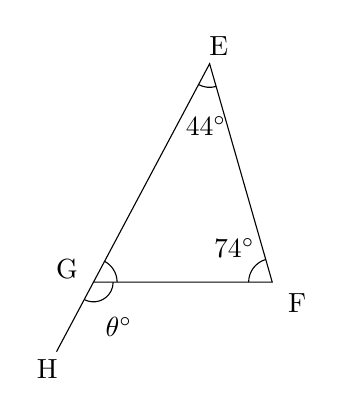
\begin{tikzpicture}[scale=1.0, baseline=(current bounding box.north)]

      \begin{scope}[rotate=242]
        \coordinate (A) at (0,0);
        \coordinate (B) at (3.1417225776930238,0);
        \coordinate (D) at (4.141722577693024,0);
        \coordinate (C) at (intersection cs: first line={(A)--($(A)+(44:4cm)$)}, second line={(B)--($(B)+(180-62:4cm)$)});
        \draw (A) -- (B) -- (C) -- cycle;
        \draw (B) -- (D);

        % Mark angles with arcs
        \draw ($(A)!0.3cm!(B)$) arc [start angle=0, end angle=44, radius=0.3cm];
        \draw ($(B)!0.3cm!(C)$) arc [start angle=180-62, end angle=180, radius=0.3cm];
        \draw ($(C)!0.3cm!(A)$) arc [start angle=180+44, end angle=360-62, radius=0.3cm];
        \draw ($(B)!0.25cm!(D)$) arc [start angle=0, end angle=180-62, radius=0.25cm];

        % Label angles
        \node at ($(A)!-0.25cm!(B)$) {E};
        \node at ($(B)!-0.45cm!(C)!0.2cm!(A)$) {G};
        \node at ($(C)!-0.25cm!(A)!-0.25cm!(B)$) {F};
        \node at ($(D)!-0.25cm!(A)$) {H};

        % Mark angles in degrees
        \coordinate (midBC) at ($(B)!0.5!(C)$);
        \node at ($(A)!0.70cm!(midBC)!0.10cm!(C)$) {$44^\circ$};

        \coordinate (midAC) at ($(A)!0.5!(C)$);
        \node at ($(B)!0.65cm!(midAC)$) {};

        \coordinate (midAB) at ($(A)!0.5!(B)$);
        \node at ($(C)!0.65cm!(midAB)$) {$74^\circ$};

        \coordinate (midDC) at ($(D)!0.3!(C)$);
        \node at ($(B)!0.65cm!(midDC)$) {$\theta^\circ$};


      \end{scope}
    \end{tikzpicture}
\end{minipage}%
\hfill
\begin{minipage}{0.4\textwidth}
  \begin{align*}
    \angle \text{HGF} &= \angle \text{E} + \angle \text{F} \\
    &= 44^\circ  + 74^\circ \\
    &= 118^\circ
  \end{align*}
\end{minipage}
\vspace{1cm} \vfill\begin{minipage}{0.55\textwidth}
  \refstepcounter{minipagecount}
  \noindent{(\theminipagecount)}\quad
  \begin{tikzpicture}[scale=1.0, baseline=(current bounding box.north)]

      \begin{scope}[rotate=177]
        \coordinate (A) at (0,0);
        \coordinate (B) at (3.933686667856967,0);
        \coordinate (D) at (4.933686667856967,0);
        \coordinate (C) at (intersection cs: first line={(A)--($(A)+(51:4cm)$)}, second line={(B)--($(B)+(180-59:4cm)$)});
        \draw (A) -- (B) -- (C) -- cycle;
        \draw (B) -- (D);

        % Mark angles with arcs
        \draw ($(A)!0.3cm!(B)$) arc [start angle=0, end angle=51, radius=0.3cm];
        \draw ($(B)!0.3cm!(C)$) arc [start angle=180-59, end angle=180, radius=0.3cm];
        \draw ($(C)!0.3cm!(A)$) arc [start angle=180+51, end angle=360-59, radius=0.3cm];
        \draw ($(B)!0.25cm!(D)$) arc [start angle=0, end angle=180-59, radius=0.25cm];

        % Label angles
        \node at ($(A)!-0.25cm!(B)$) {E};
        \node at ($(B)!-0.45cm!(C)!0.2cm!(A)$) {F};
        \node at ($(C)!-0.25cm!(A)!-0.25cm!(B)$) {G};
        \node at ($(D)!-0.25cm!(A)$) {H};

        % Mark angles in degrees
        \coordinate (midBC) at ($(B)!0.5!(C)$);
        \node at ($(A)!0.70cm!(midBC)!0.10cm!(C)$) {$51^\circ$};

        \coordinate (midAC) at ($(A)!0.5!(C)$);
        \node at ($(B)!0.65cm!(midAC)$) {};

        \coordinate (midAB) at ($(A)!0.5!(B)$);
        \node at ($(C)!0.65cm!(midAB)$) {$70^\circ$};

        \coordinate (midDC) at ($(D)!0.3!(C)$);
        \node at ($(B)!0.65cm!(midDC)$) {$\theta^\circ$};


      \end{scope}
    \end{tikzpicture}
\end{minipage}%
\hfill
\begin{minipage}{0.4\textwidth}
  \begin{align*}
    \angle \text{HFG} &= \angle \text{E} + \angle \text{G} \\
    &= 51^\circ  + 70^\circ \\
    &= 121^\circ
  \end{align*}
\end{minipage}
\vspace{1cm} \vfill\begin{minipage}{0.55\textwidth}
  \refstepcounter{minipagecount}
  \noindent{(\theminipagecount)}\quad
  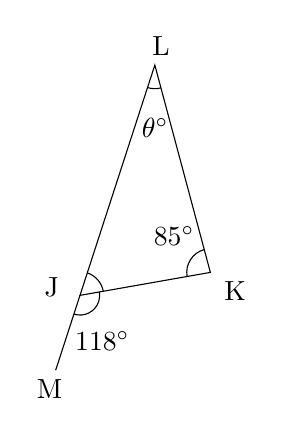
\begin{tikzpicture}[scale=1.0, baseline=(current bounding box.north)]

      \begin{scope}[rotate=252]
        \coordinate (A) at (0,0);
        \coordinate (B) at (3.0750475049344095,0);
        \coordinate (D) at (4.0750475049344095,0);
        \coordinate (C) at (intersection cs: first line={(A)--($(A)+(33:4cm)$)}, second line={(B)--($(B)+(180-62:4cm)$)});
        \draw (A) -- (B) -- (C) -- cycle;
        \draw (B) -- (D);

        % Mark angles with arcs
        \draw ($(A)!0.3cm!(B)$) arc [start angle=0, end angle=33, radius=0.3cm];
        \draw ($(B)!0.3cm!(C)$) arc [start angle=180-62, end angle=180, radius=0.3cm];
        \draw ($(C)!0.3cm!(A)$) arc [start angle=180+33, end angle=360-62, radius=0.3cm];
        \draw ($(B)!0.25cm!(D)$) arc [start angle=0, end angle=180-62, radius=0.25cm];

        % Label angles
        \node at ($(A)!-0.25cm!(B)$) {L};
        \node at ($(B)!-0.45cm!(C)!0.2cm!(A)$) {J};
        \node at ($(C)!-0.25cm!(A)!-0.25cm!(B)$) {K};
        \node at ($(D)!-0.25cm!(A)$) {M};

        % Mark angles in degrees
        \coordinate (midBC) at ($(B)!0.5!(C)$);
        \node at ($(A)!0.70cm!(midBC)!0.10cm!(C)$) {$\theta^\circ$};

        \coordinate (midAC) at ($(A)!0.5!(C)$);
        \node at ($(B)!0.65cm!(midAC)$) {};

        \coordinate (midAB) at ($(A)!0.5!(B)$);
        \node at ($(C)!0.65cm!(midAB)$) {$85^\circ$};

        \coordinate (midDC) at ($(D)!0.3!(C)$);
        \node at ($(B)!0.65cm!(midDC)$) {$118^\circ$};


      \end{scope}
    \end{tikzpicture}
\end{minipage}%
\hfill
\begin{minipage}{0.4\textwidth}
  \begin{align*}
    \angle \text{L} &= \angle \text{MJK} - \angle \text{K} \\
    &= 118^\circ  - 85^\circ \\
    &= 33^\circ
  \end{align*}
\end{minipage}
\vspace{1cm} \vfill\pagebreak ~ \newline ~ \newline\begin{minipage}{0.55\textwidth}
  \refstepcounter{minipagecount}
  \noindent{(\theminipagecount)}\quad
  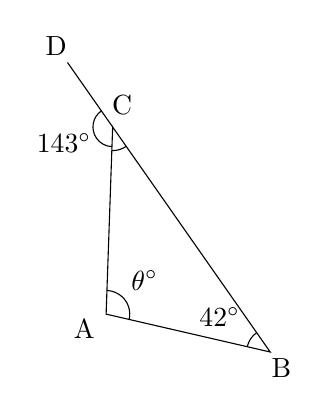
\begin{tikzpicture}[scale=1.0, baseline=(current bounding box.north)]

      \begin{scope}[rotate=125]
        \coordinate (A) at (0,0);
        \coordinate (B) at (3.488914166811965,0);
        \coordinate (D) at (4.4889141668119645,0);
        \coordinate (C) at (intersection cs: first line={(A)--($(A)+(42:4cm)$)}, second line={(B)--($(B)+(180-37:4cm)$)});
        \draw (A) -- (B) -- (C) -- cycle;
        \draw (B) -- (D);

        % Mark angles with arcs
        \draw ($(A)!0.3cm!(B)$) arc [start angle=0, end angle=42, radius=0.3cm];
        \draw ($(B)!0.3cm!(C)$) arc [start angle=180-37, end angle=180, radius=0.3cm];
        \draw ($(C)!0.3cm!(A)$) arc [start angle=180+42, end angle=360-37, radius=0.3cm];
        \draw ($(B)!0.25cm!(D)$) arc [start angle=0, end angle=180-37, radius=0.25cm];

        % Label angles
        \node at ($(A)!-0.25cm!(B)$) {B};
        \node at ($(B)!-0.45cm!(C)!0.2cm!(A)$) {C};
        \node at ($(C)!-0.25cm!(A)!-0.25cm!(B)$) {A};
        \node at ($(D)!-0.25cm!(A)$) {D};

        % Mark angles in degrees
        \coordinate (midBC) at ($(B)!0.5!(C)$);
        \node at ($(A)!0.70cm!(midBC)!0.10cm!(C)$) {$42^\circ$};

        \coordinate (midAC) at ($(A)!0.5!(C)$);
        \node at ($(B)!0.65cm!(midAC)$) {};

        \coordinate (midAB) at ($(A)!0.5!(B)$);
        \node at ($(C)!0.65cm!(midAB)$) {$\theta^\circ$};

        \coordinate (midDC) at ($(D)!0.3!(C)$);
        \node at ($(B)!0.65cm!(midDC)$) {$143^\circ$};


      \end{scope}
    \end{tikzpicture}
\end{minipage}%
\hfill
\begin{minipage}{0.4\textwidth}
  \begin{align*}
    \angle \text{A} &= \angle \text{DCA} - \angle \text{B} \\
    &= 143^\circ  - 42^\circ \\
    &= 101^\circ
  \end{align*}
\end{minipage}
\vspace{1cm} \vfill\begin{minipage}{0.55\textwidth}
  \refstepcounter{minipagecount}
  \noindent{(\theminipagecount)}\quad
  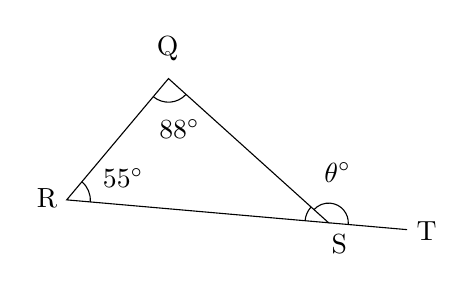
\begin{tikzpicture}[scale=1.0, baseline=(current bounding box.north)]

      \begin{scope}[rotate=355]
        \coordinate (A) at (0,0);
        \coordinate (B) at (3.339240762027264,0);
        \coordinate (D) at (4.339240762027265,0);
        \coordinate (C) at (intersection cs: first line={(A)--($(A)+(55:4cm)$)}, second line={(B)--($(B)+(180-37:4cm)$)});
        \draw (A) -- (B) -- (C) -- cycle;
        \draw (B) -- (D);

        % Mark angles with arcs
        \draw ($(A)!0.3cm!(B)$) arc [start angle=0, end angle=55, radius=0.3cm];
        \draw ($(B)!0.3cm!(C)$) arc [start angle=180-37, end angle=180, radius=0.3cm];
        \draw ($(C)!0.3cm!(A)$) arc [start angle=180+55, end angle=360-37, radius=0.3cm];
        \draw ($(B)!0.25cm!(D)$) arc [start angle=0, end angle=180-37, radius=0.25cm];

        % Label angles
        \node at ($(A)!-0.25cm!(B)$) {R};
        \node at ($(B)!-0.45cm!(C)!0.2cm!(A)$) {S};
        \node at ($(C)!-0.25cm!(A)!-0.25cm!(B)$) {Q};
        \node at ($(D)!-0.25cm!(A)$) {T};

        % Mark angles in degrees
        \coordinate (midBC) at ($(B)!0.5!(C)$);
        \node at ($(A)!0.70cm!(midBC)!0.10cm!(C)$) {$55^\circ$};

        \coordinate (midAC) at ($(A)!0.5!(C)$);
        \node at ($(B)!0.65cm!(midAC)$) {};

        \coordinate (midAB) at ($(A)!0.5!(B)$);
        \node at ($(C)!0.65cm!(midAB)$) {$88^\circ$};

        \coordinate (midDC) at ($(D)!0.3!(C)$);
        \node at ($(B)!0.65cm!(midDC)$) {$\theta^\circ$};


      \end{scope}
    \end{tikzpicture}
\end{minipage}%
\hfill
\begin{minipage}{0.4\textwidth}
  \begin{align*}
    \angle \text{TSQ} &= \angle \text{R} + \angle \text{Q} \\
    &= 55^\circ  + 88^\circ \\
    &= 143^\circ
  \end{align*}
\end{minipage}
\vspace{1cm} \vfill\begin{minipage}{0.55\textwidth}
  \refstepcounter{minipagecount}
  \noindent{(\theminipagecount)}\quad
  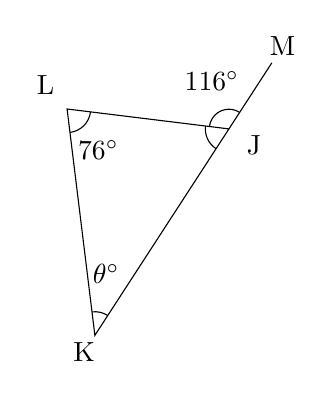
\begin{tikzpicture}[scale=1.0, baseline=(current bounding box.north)]

      \begin{scope}[rotate=57]
        \coordinate (A) at (0,0);
        \coordinate (B) at (3.126090187879801,0);
        \coordinate (D) at (4.126090187879801,0);
        \coordinate (C) at (intersection cs: first line={(A)--($(A)+(40:4cm)$)}, second line={(B)--($(B)+(180-64:4cm)$)});
        \draw (A) -- (B) -- (C) -- cycle;
        \draw (B) -- (D);

        % Mark angles with arcs
        \draw ($(A)!0.3cm!(B)$) arc [start angle=0, end angle=40, radius=0.3cm];
        \draw ($(B)!0.3cm!(C)$) arc [start angle=180-64, end angle=180, radius=0.3cm];
        \draw ($(C)!0.3cm!(A)$) arc [start angle=180+40, end angle=360-64, radius=0.3cm];
        \draw ($(B)!0.25cm!(D)$) arc [start angle=0, end angle=180-64, radius=0.25cm];

        % Label angles
        \node at ($(A)!-0.25cm!(B)$) {K};
        \node at ($(B)!-0.45cm!(C)!0.2cm!(A)$) {J};
        \node at ($(C)!-0.25cm!(A)!-0.25cm!(B)$) {L};
        \node at ($(D)!-0.25cm!(A)$) {M};

        % Mark angles in degrees
        \coordinate (midBC) at ($(B)!0.5!(C)$);
        \node at ($(A)!0.70cm!(midBC)!0.10cm!(C)$) {$\theta^\circ$};

        \coordinate (midAC) at ($(A)!0.5!(C)$);
        \node at ($(B)!0.65cm!(midAC)$) {};

        \coordinate (midAB) at ($(A)!0.5!(B)$);
        \node at ($(C)!0.65cm!(midAB)$) {$76^\circ$};

        \coordinate (midDC) at ($(D)!0.3!(C)$);
        \node at ($(B)!0.65cm!(midDC)$) {$116^\circ$};


      \end{scope}
    \end{tikzpicture}
\end{minipage}%
\hfill
\begin{minipage}{0.4\textwidth}
  \begin{align*}
    \angle \text{K} &= \angle \text{MJL} - \angle \text{L} \\
    &= 116^\circ  - 76^\circ \\
    &= 40^\circ
  \end{align*}
\end{minipage}
\vspace{1cm} \vfill\begin{minipage}{0.55\textwidth}
  \refstepcounter{minipagecount}
  \noindent{(\theminipagecount)}\quad
  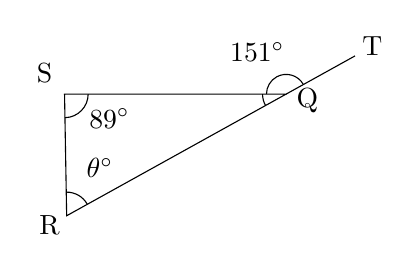
\begin{tikzpicture}[scale=1.0, baseline=(current bounding box.north)]

      \begin{scope}[rotate=29]
        \coordinate (A) at (0,0);
        \coordinate (B) at (3.1874698343428696,0);
        \coordinate (D) at (4.18746983434287,0);
        \coordinate (C) at (intersection cs: first line={(A)--($(A)+(62:4cm)$)}, second line={(B)--($(B)+(180-29:4cm)$)});
        \draw (A) -- (B) -- (C) -- cycle;
        \draw (B) -- (D);

        % Mark angles with arcs
        \draw ($(A)!0.3cm!(B)$) arc [start angle=0, end angle=62, radius=0.3cm];
        \draw ($(B)!0.3cm!(C)$) arc [start angle=180-29, end angle=180, radius=0.3cm];
        \draw ($(C)!0.3cm!(A)$) arc [start angle=180+62, end angle=360-29, radius=0.3cm];
        \draw ($(B)!0.25cm!(D)$) arc [start angle=0, end angle=180-29, radius=0.25cm];

        % Label angles
        \node at ($(A)!-0.25cm!(B)$) {R};
        \node at ($(B)!-0.45cm!(C)!0.2cm!(A)$) {Q};
        \node at ($(C)!-0.25cm!(A)!-0.25cm!(B)$) {S};
        \node at ($(D)!-0.25cm!(A)$) {T};

        % Mark angles in degrees
        \coordinate (midBC) at ($(B)!0.5!(C)$);
        \node at ($(A)!0.70cm!(midBC)!0.10cm!(C)$) {$\theta^\circ$};

        \coordinate (midAC) at ($(A)!0.5!(C)$);
        \node at ($(B)!0.65cm!(midAC)$) {};

        \coordinate (midAB) at ($(A)!0.5!(B)$);
        \node at ($(C)!0.65cm!(midAB)$) {$89^\circ$};

        \coordinate (midDC) at ($(D)!0.3!(C)$);
        \node at ($(B)!0.65cm!(midDC)$) {$151^\circ$};


      \end{scope}
    \end{tikzpicture}
\end{minipage}%
\hfill
\begin{minipage}{0.4\textwidth}
  \begin{align*}
    \angle \text{R} &= \angle \text{TQS} - \angle \text{S} \\
    &= 151^\circ  - 89^\circ \\
    &= 62^\circ
  \end{align*}
\end{minipage}
\vspace{1cm} \vfill

\end{document}
